\chapter{Simulation flow chart}

This section is intended to provide a description of the simulation flow chart. In particular, a special focus will be given to the user's point of view (i.e. necessary input to provide and choices to make) when launching a simulation, and to the model point of view (i.e. calculation flow chart).

\section{User point of view}
The user that needs to fulfill a set of tasks in order to prepare the input necessary to launch a GEOtop simulation, as reported in Fig. \ref{Fig_sim_flowchart}.

\paragraph{Set general parameters}
 The user must define the type of simulation (1D or 3D) and other general input.

\paragraph{Meteo station characterization}
The user must define the position and characteristics of the meteo stations.

\paragraph{Meteo data}
The user must define the meteorological forcing measured in each meteo station.

\paragraph{Topographic characterization}
The user must define the topographical characteristics of the domain area (i.e. elevation, aspect, slope, sky view factor, curvature).

\paragraph{Land cover characterization}
The user must define the surface type characteristics of the domain (often called ``land use'' or ``land cover'').

\paragraph{Soil type characterization}
The user must define the soil type characteristics of the domain area (i.e. soil texture, soil water retention curve etc.).

\paragraph{Initial conditions}
The user must define the initial temperature and water content in each cell of the domain.

\paragraph{Boundary conditions}
The user must define the behavior (fluxes) at the border domain.

\paragraph{Physical parameters}
The user must parametrize the various physical processes involved. In particular, the current version of GEOtop allow to specify the parameters typical of the following processes: glacier, snow, vegetation, soil/rock thermal, soil/rock hydraulic and discharge).

\paragraph{Output parameters}
The user must determine the desired information to be printed and the correspondent frequency.



\begin{figure}[!h]
\centering
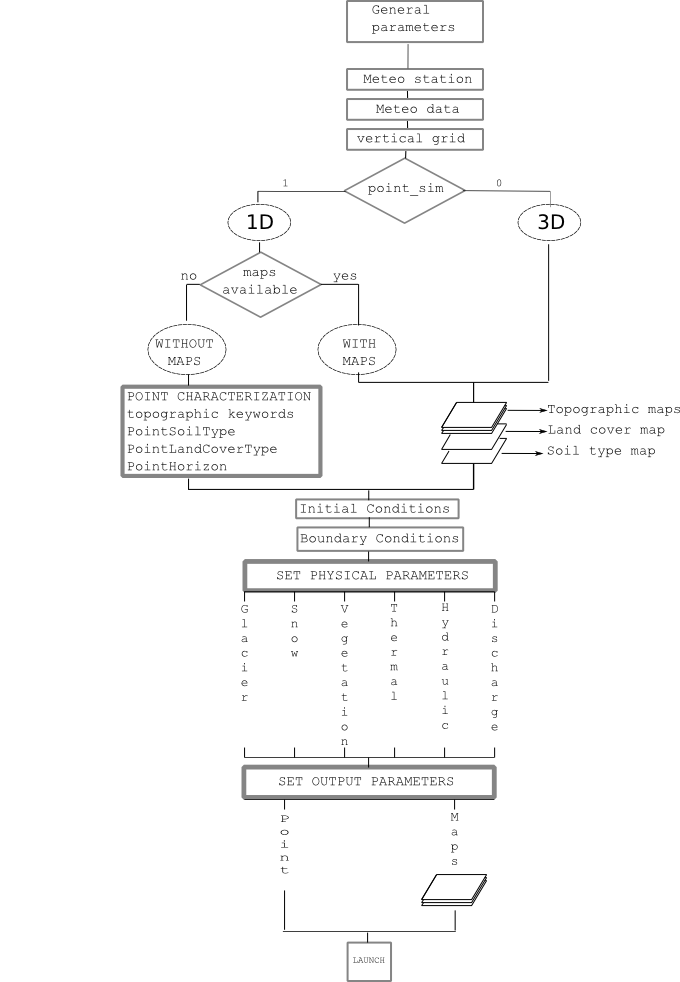
\includegraphics[height=0.8\textheight]{./images/pic_flowchart/SCHEMAi.png}
\caption{GEOtop flow chart: user point of view for preparing a simulation}
\label{Fig_sim_flowchart}
\end{figure}


\begin{table}[!h]
\begin{center}
\begin{minipage}[c]{0.42\textwidth}
\begin{tabular}{c|c}
HeaderHorizonAngle & HeaderHorizonHeight\\
``azi'' & ``hang''\\
\hline
45 \textdegree	&	0.00\\
135 \textdegree	&	10.00\\
225 \textdegree	& 	30.00\\
315 \textdegree	&	5.00\\
\hline
\end{tabular}
\end{minipage}
\hspace{0.5cm}
\begin{minipage}[c]{0.42\textwidth}
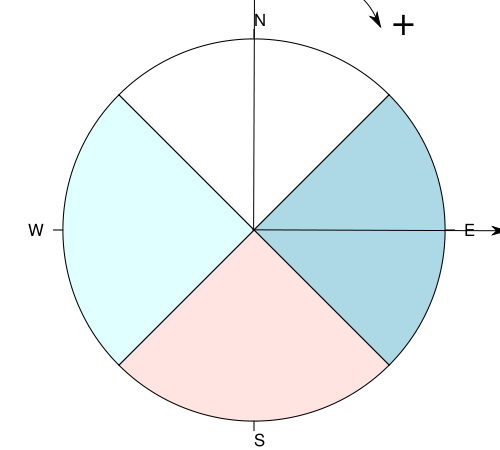
\includegraphics[width=1\textwidth]{./images/pic_1D/pie.png} 
\end{minipage}
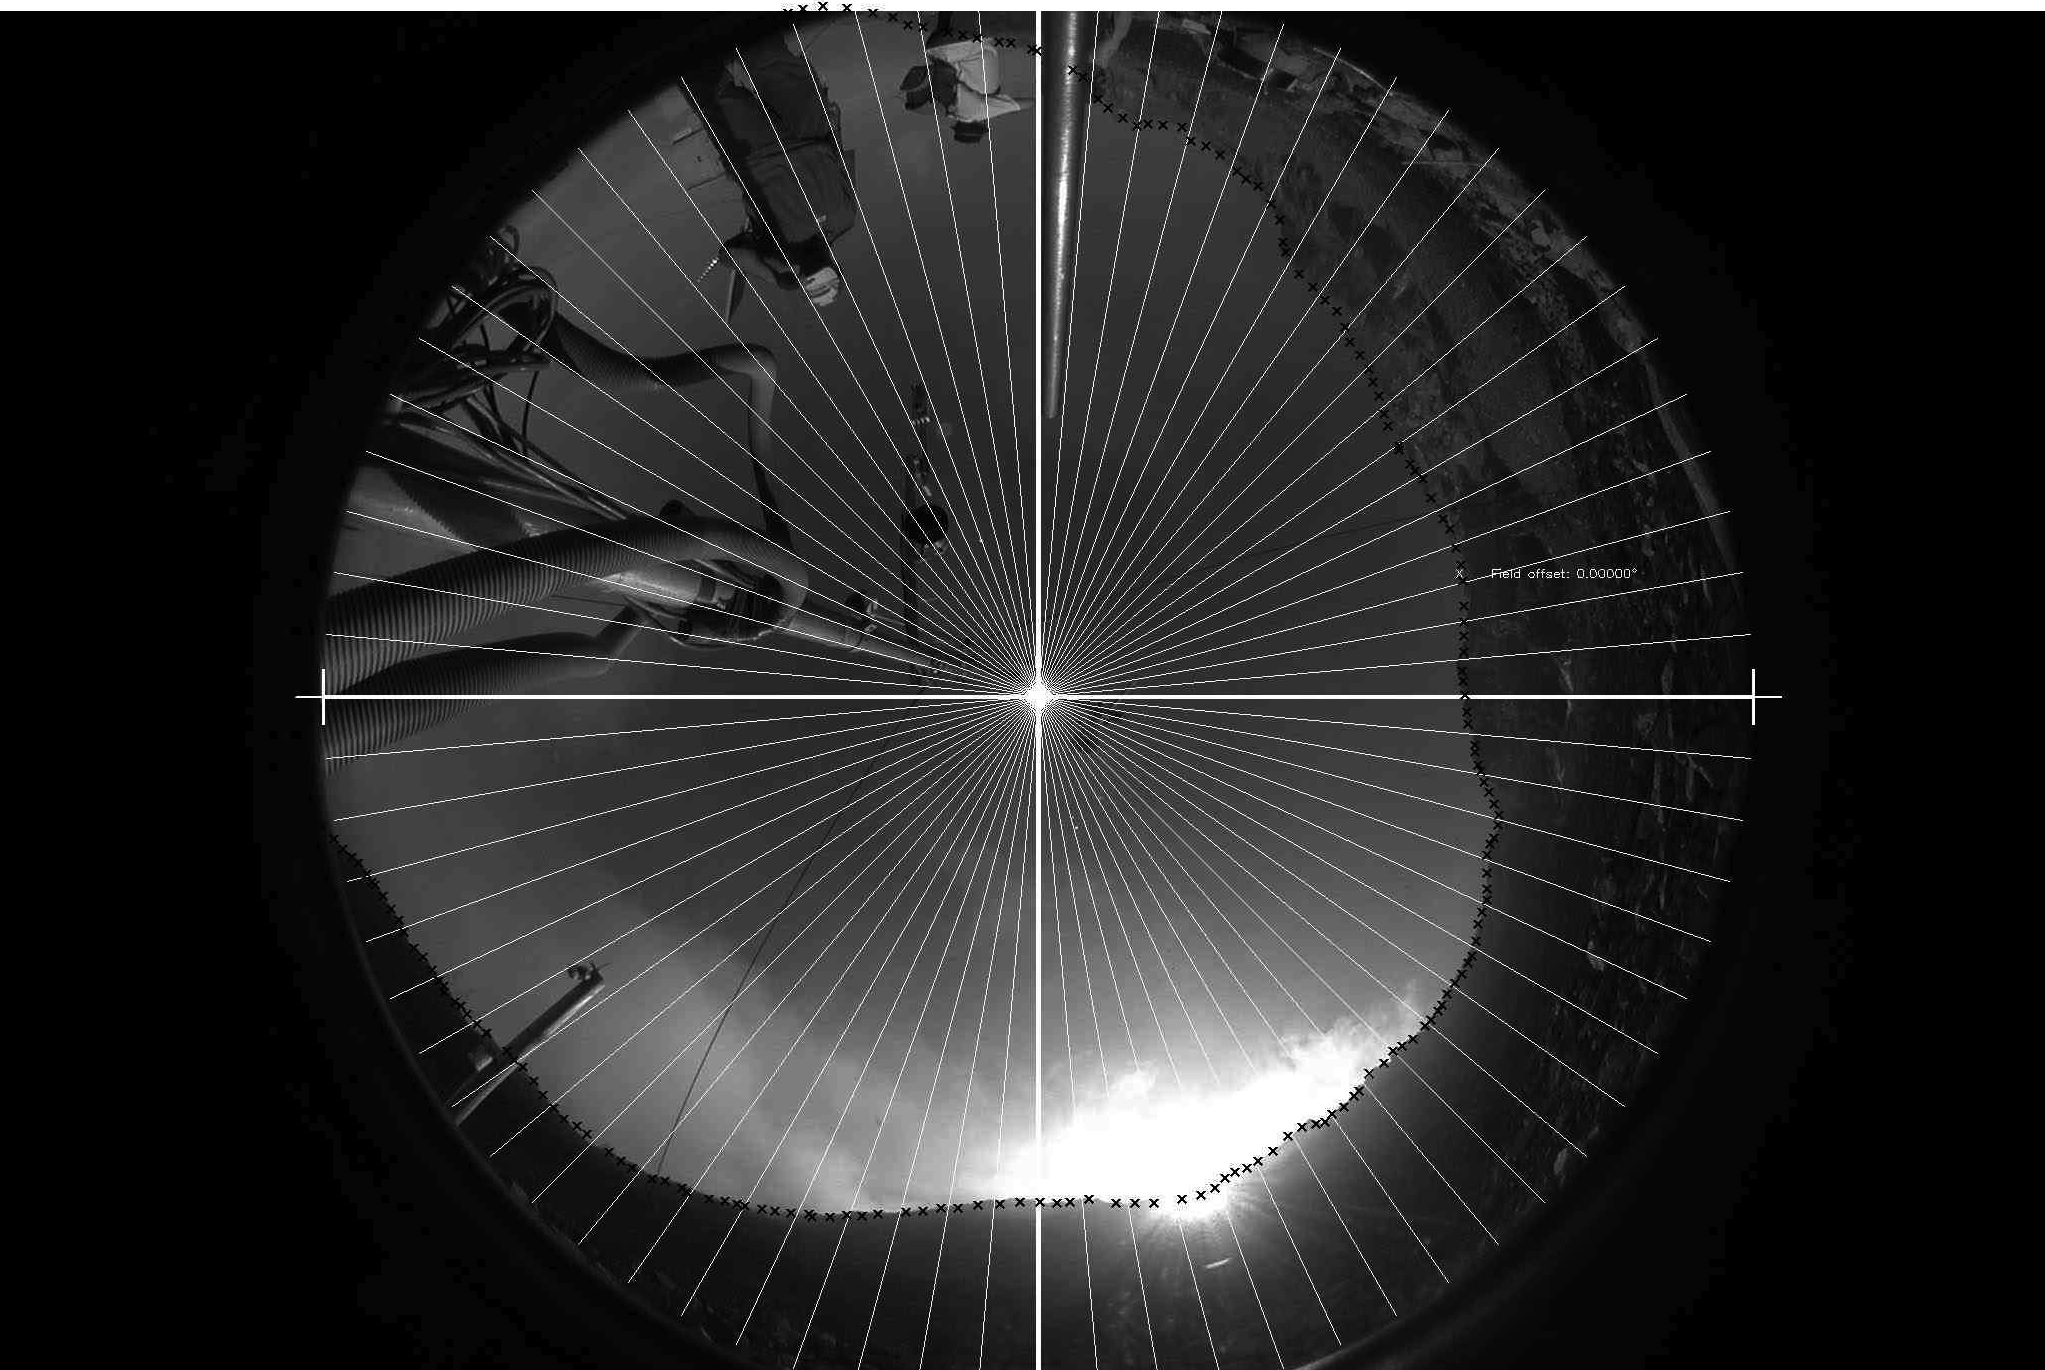
\includegraphics[width=0.8\textwidth]{./images/pic_1D/fish_eye_view.jpg}
\textsl{\caption{Top: example of the default horizon file and of the corresponding azimuth classes. An example is given in Par. \ref{Par_keyprop}. Bottom: example of a fish-eye view from a point (courtesy of Stephan Gruber)}
\label{azh}}
\end{center}
\end{table}

\section{1D simulations}\label{par:1D3D}

Originally GEOtop was born as a hydrological model with the objective to produce maps of hydrological variables in a catchment. Later, thanks to the boost received by the permafrost community, it was adapted also to analyze single points located in extreme topographies. In these points, as outlined in Par. \ref{par:focusPoints}, for various reasons it may be interesting to produce 1D simulations. In fact 1D simulations are often useful as they allow to obtain results very rapidly and, in some cases, sufficiently reliable. 

%=============================================================%
\subsection{Point horizon}\label{descr_horizon}
%=============================================================%

In order to account for the topography visible by the simulation point, it is recommendable to provide the horizon file of the point.
Every point $P(x,y,z)$ on the landscape, unless in the middle of a flat terrain, is surrounded by obstacles like mountains, buildings, trees. These objects, during the day, according to the elevation and position (azimuth) of the sun at a particular time in the year (julian day and day time), may produce a cast shadow on the point $P$ that prevents the point from receiving direct solar radiation. \\
Thanks to proper cameras (e.g. fish-eye camera, see bottom of Fig. \ref{azh}) or to GIS routines, it is possible to produce a file that outlines the angle height of the obstacles along a given azimuth direction.
The {\it HorizonPointFile} \index{HorizonPointFile} allows to specify the horizon seen by a point $P$ along a desired discretization of the azimuth. The file structure is thus a matrix whose first column represents the azimuth angle and the second column the elevation angle of the object height. The Table \ref{azh}) reports the horizon file where the azimuth has been discretized in 4 parts. Note that the North direction must always be in the center of the slides in which the circle is divided. It is possible to increase the azimuth classes in order to provide a more detailed description of the obstacles height.\\
The horizon data may be specified in the following cases:
\begin{enumerate}
 \item 1D simulations: since the topography is not provided, the user may provide the horizon file for every simulated point. 
Unless given, the model creates one assuming an overall flat terrain;
 \item for meteorological stations: in this case it is needed to set the time when the sun is obscured by the obstacle; from that time onward the cloudiness calculation is no more carried by the ratio between actual and potential radiation, since the actual radiation would no longer provide a reliable value.
\end{enumerate}

\subsection{1D simulations: with or without maps}\label{}

Let us suppose to select five points in the basin (see Fig. \ref{grid3Dversante_points}) where we want to run five 1D simulations. First of all it is necessary to provide the coordinates (X, Y) of the points, together with the average latitude and longitude of the area. In addition to that, it is necessary to characterize the points by specifying the topography (elevation, aspect, slope, sky view factor, curvatures and the horizon), the soil type and land cover.  This last information may be provided in two ways:
\begin{itemize}
\item {\bf with maps}: the topographical, land cover and soil type maps are provided and the model, according to the coordinates of the points, automatically sets the topographical characteristics;
\item {\bf without maps}: the user has to specify all the characteristics of the points (e.g. see Table \ref{table_in_topochar}).
\end{itemize}

\subsection{1D simulations in steep topography}\label{}

The domain scheme of a 1D simulation at steep mountain topography is depicted in Fig. \ref{Fig_1Dsteep}: the scheme is represented on the left: the axis of elevation $Z_f$ is on the vertical direction and sets the elevation of the point on the surface, whereas the layers are located normal to the slope. If present, also the slope, aspect and horizon of the point $P_1$ may be specified. 
As the 1D representation is just an abstract sequence of layers of various depths located along on an imaginary line, one may think that the final scheme resembles what outlined on the right, where the elevation axis and the line $Z$ axis form an angle complementary to the slope angle. Note that the $Z$ axis does not coincide with the gravitational $Z_f$ axis.
\begin{figure}[t]
\centering
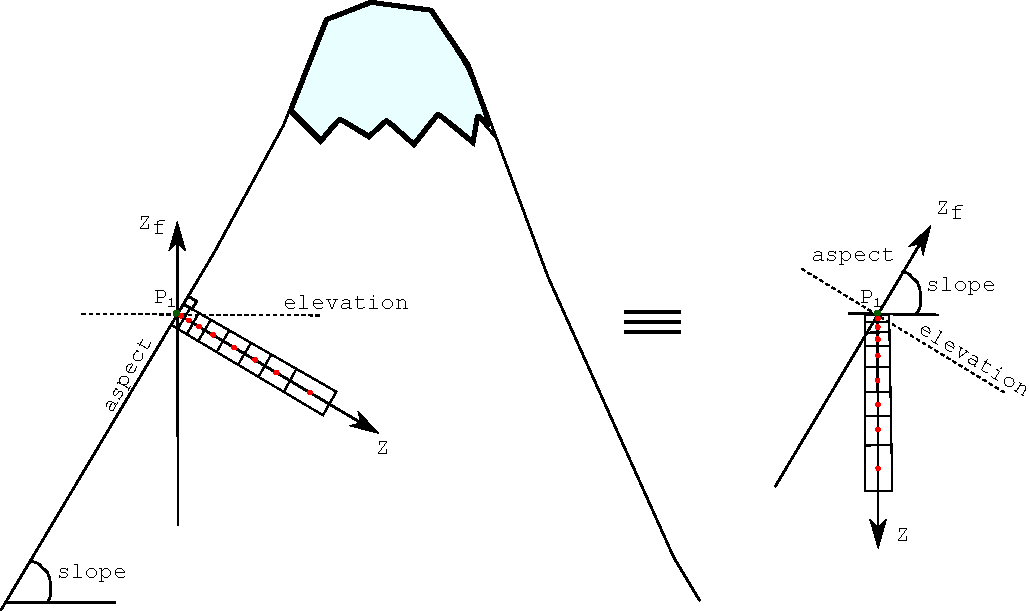
\includegraphics[width=0.85\textwidth]{./images/pic_flowchart/1Dsimul.pdf}
\caption{Scheme of a 1D simulation on steep topography typical of high mountain altitude}
\label{Fig_1Dsteep}
\end{figure}

\section{Model point of view}
 On the other hand, the model transforms the input given by the user into results, by solving the energy and mass balance in the calculation domain. As reported in Fig. \ref{Fig_sim_flowchart2}, at the beginning of the simulation, GEOtop does the following activities: 
\paragraph{1. Read input data} In this phase, the model reads: (i) the keywords and parameters specified in {\it geotop.inpts} and other properly defined files; (ii) the topographic maps (elevation, aspect, slope, sky view factor, curvature), the land cover map (that coincides with the calculation mask), the map of soil type and, if available, the maps of initial conditions; (iii) reads the parameters (physical and output). If a parameter or a map is not specified with the proper keyword, it assumes the default value.

\paragraph{2. Create and initialize mesh} As reported in Par. \ref{Par:calc_grid}, it creates the calculation mesh according to the grid size of the land cover map and the vertical nodes spacing defined for the vertical grid. Then it initializes the temperature and water pressure head of each node with the initial conditions and sets the physical parameters according to what specified by the keywords. 

\paragraph{3. Read meteo data} During this phase it incorporates the meteorological data for each meteo station: these data represent the forcing that will drive the simulation, producing the dynamic boundary conditions for the surface nodes. Finally, GEOtop sets the initial simulation time to initialize the simulation counter: this will allow to compare the current simulation time with the expected simulation end time. \\

\noindent At this point begins the time loop for the calculation and the printing routines. In particular, at each calculation time step, GEOtop fulfills the following tasks:
\paragraph {1. Distribute meteorological forcing}
This allows to spatially distribute the meteorological forcing, measured in discrete meteo station, in all the calculation cells. This methodology is based on \citet{liston2006meteorological}.

\paragraph{2. Energy balance}
In this phase the energy balance equation is solved. This encompasses the calculation of the surface energy fluxes, the vegetation module, the snow/glacier module and the routine that the calculates the soil temperatures and ice content.

\paragraph{3. Water balance}
In this phase the mass balance equation is solved. This encompasses the calculation of the infiltration routine to determine the pore water pressure and water content through a 3D Richards solver. Eventually, the runoff and channel routing routines, based on a shallow-water solver, will allow to determine the discharge at the basin outlet.

\paragraph{4. Write output}
This phase is intended to print the point information and the maps according to the desired output frequency.

\paragraph{5. Update and check time}
This phase updates the time with the calculation time step and compares the new time with the simulation end time, to verify whether to stop the simulation or loop again. If the current simulation time exceeds the end of the simulation, then the program stops and deallocates all the structures.


\begin{figure}[t]
\centering
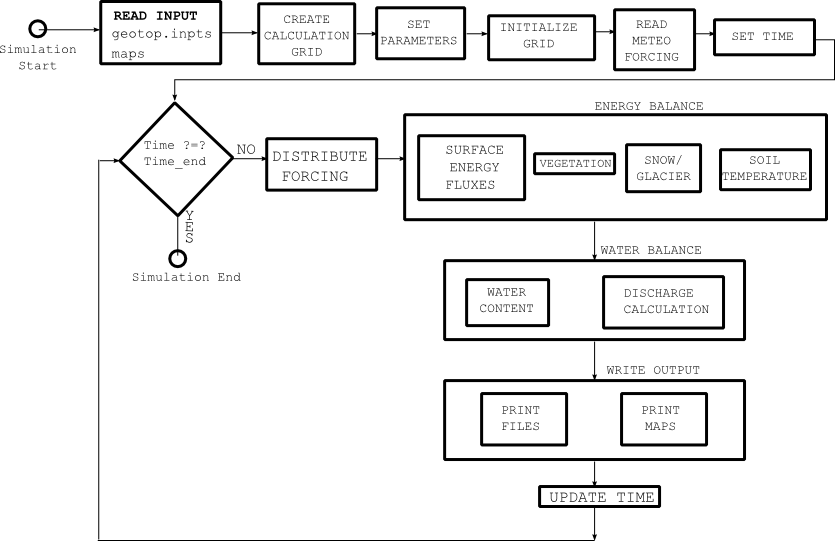
\includegraphics[width=0.9\textwidth]{./images/pic_flowchart/SCHEMAii.png}
\caption{GEOtop flow chart: model point of view for accomplishing a simulation}
\label{Fig_sim_flowchart2}
\end{figure}


\newpage
\section{How to Run GEOtop}
%%%%%%%%%%%%%%%%%%%%%%%%%%%%%%%%%%%%%%%%%%%%%%%%%%%%%%%%%%%%%%%
\subsection{From Terminal}

\noindent Open a terminal, go into the folder \textsl{Debug} by typing:

\footnotesize{
\begin{verbatim}
$ cd Debug
\end{verbatim}
}

\noindent Write:

\footnotesize{
\begin{verbatim}
$ ./GEOtop1.2 
\end{verbatim}
}

\noindent Leave one space and type now the path to the folder where the simulation files are:

\footnotesize{
\begin{verbatim}
$./GEOtop_1.2 /Users/matteo/Duron/
\end{verbatim}
}

\noindent Remember to put a``/'' (slash) at the end and the type {\it Return}. The simulation should start.


\begin{figure}[!h]
\begin{center}
  \begin{minipage}[c]{.8\textwidth}
    \centering
    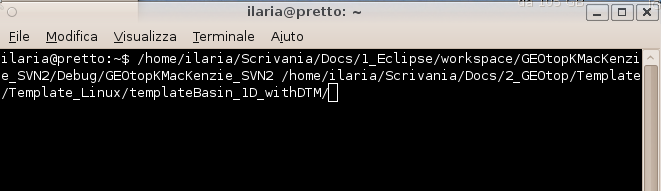
\includegraphics[width=0.9\textwidth]{./images/pic_flowchart/13_terminale_trim.png}
  \end{minipage}
\end{center}
    \textsl{\caption{SVN} \label{f:10}}
\end{figure}

\begin{figure}[!h]
\begin{center}
  \begin{minipage}[c]{.8\textwidth}
    \centering
    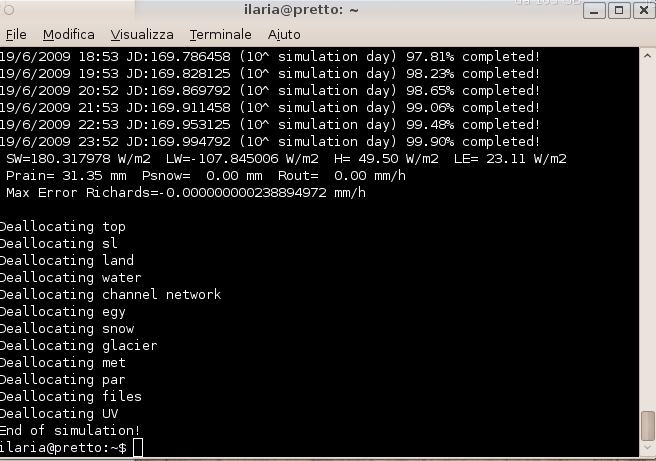
\includegraphics[width=0.9\textwidth]{./images/pic_flowchart/13_terminale_end.png}
  \end{minipage}
\end{center}
    \textsl{\caption{SVN} \label{f:10}}
\end{figure}




%\subsection{From Eclipse}
%\begin{itemize}
% \item \textsl{Run} $\rightarrow$ \textsl{Run Configurations}
% \item Click on the icon: \textsl{New launch configuration}
% \item \textsl{C/C++ Applications} $\rightarrow$ click on \textsl{'New configuration'}
% \item \textsl{Name} $\rightarrow$ Choose a name you like for the project, as for example: GEOtop
% \item \textsl{Arguments} $\rightarrow$ \textsl{Program Arguments} $\rightarrow$ \textsl{Type} ./
% \item \textsl{Working directory} $\rightarrow$ Uncheck the \textsl{'Use default'} string 
% \item \textsl{Working directory} $\rightarrow$ Click on 'File System' $\rightarrow$ Select the path of the folder
%containing the input files for the simulation 
% \item Click on \textsl{'Apply'} button
% \item Click on \textsl{'Run'} button
%\end{itemize}


%\begin{figure}[!h]
%\begin{center}
%  \begin{minipage}[c]{.45\textwidth}
%    \centering
%    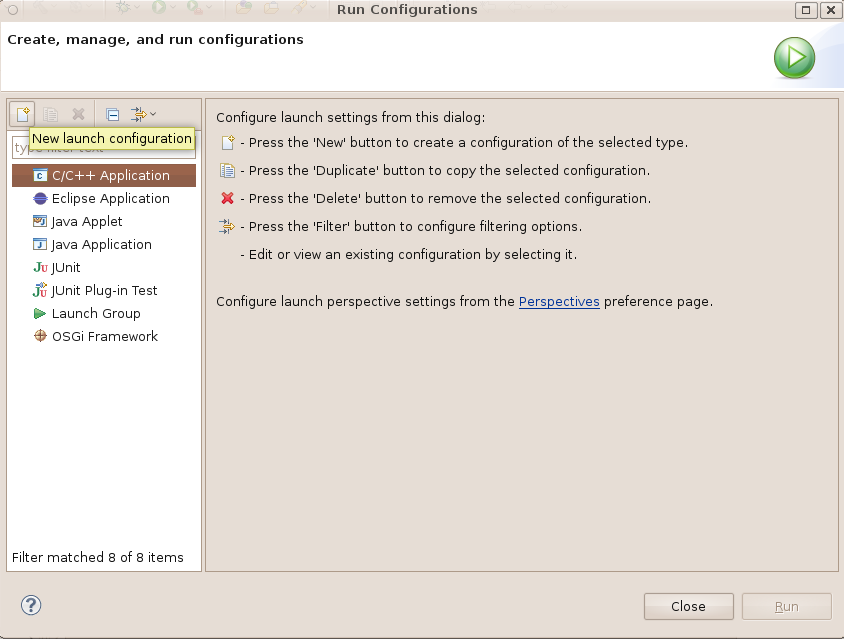
\includegraphics[width=1\textwidth]{./images/pic_compile/10_run_0.png}
%  \end{minipage}
%  \begin{minipage}[c]{.45\textwidth}
%    \centering
%    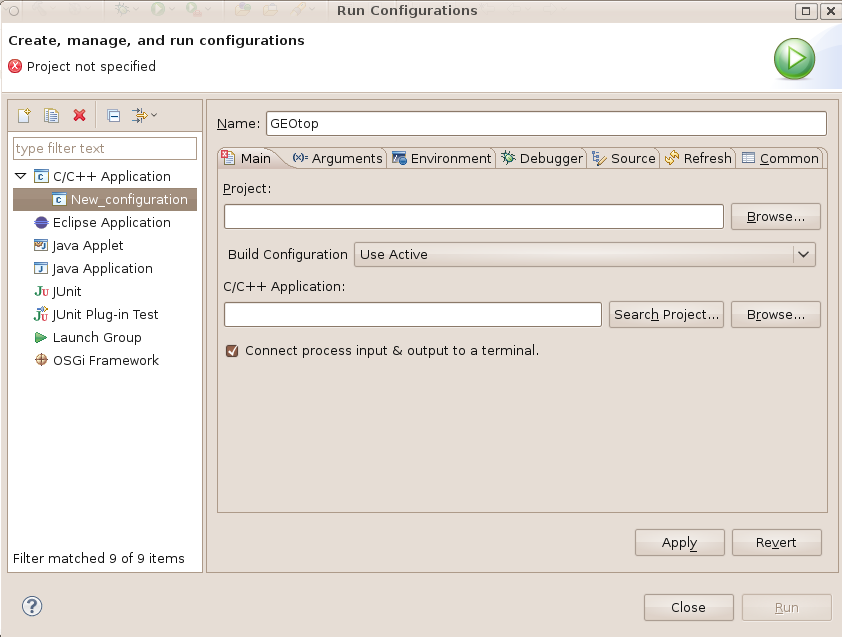
\includegraphics[width=1\textwidth]{./images/pic_compile/10_run_1.png}
%  \end{minipage}
%\end{center}
%    \textsl{\caption{SVN} \label{f:9_1}}
%\end{figure}


%\begin{figure}[!h]
%\begin{center}
%  \begin{minipage}[c]{.45\textwidth}
%    \centering
%    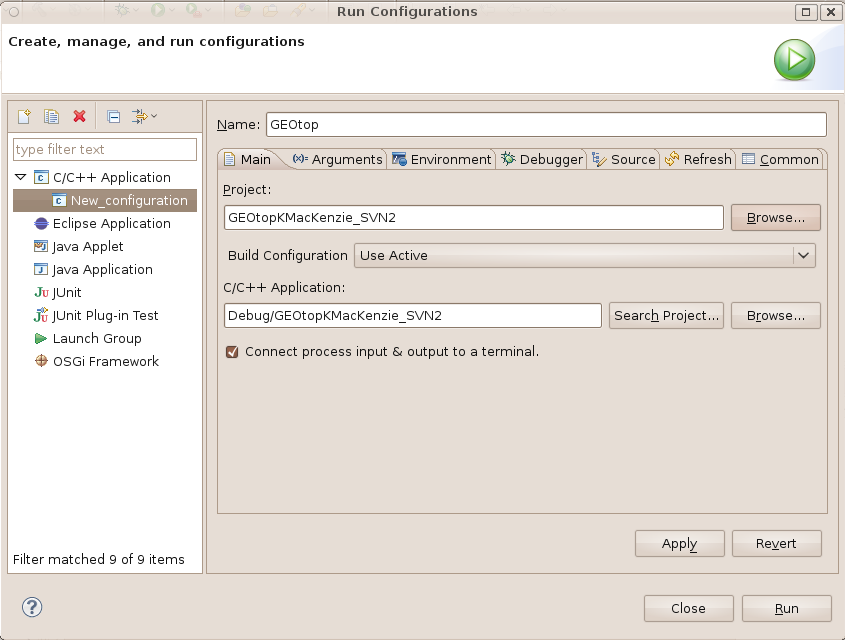
\includegraphics[width=1\textwidth]{./images/pic_compile/10_run_2.png}
%  \end{minipage}
%  \begin{minipage}[c]{.45\textwidth}
%    \centering
%    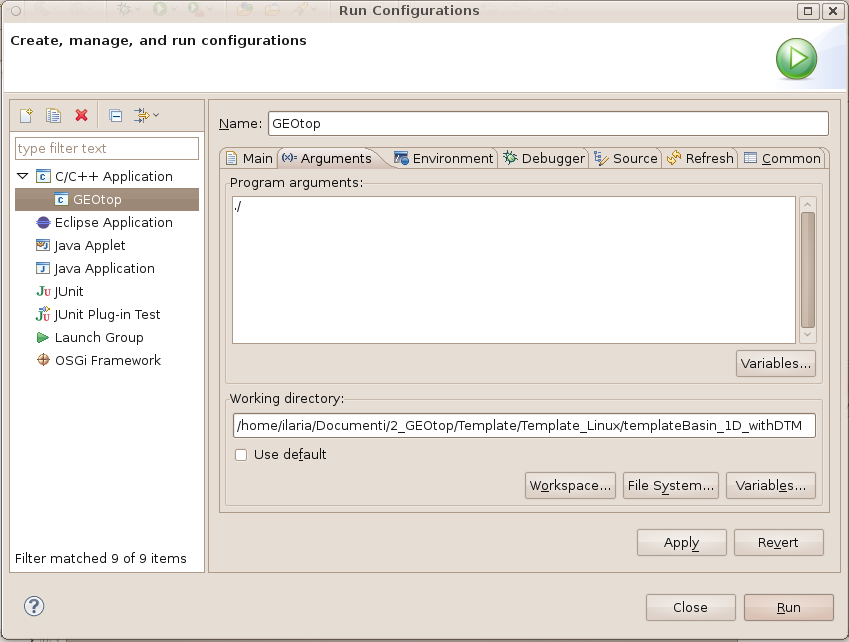
\includegraphics[width=1\textwidth]{./images/pic_compile/10_run_3.png}
%  \end{minipage}
%\end{center}
%    \textsl{\caption{SVN} \label{f:9_2}}
%\end{figure}

